
\documentclass[a4paper,twocolumn]{article}
\usepackage{graphicx}
\usepackage[T1]{fontenc}
\usepackage[utf8]{inputenc}
\usepackage{amssymb}
\usepackage[utf8]{inputenc} 
\usepackage{cite} 
\usepackage[final]{hyperref}
\usepackage[swedish,english]{babel}
\usepackage{amsmath}
\usepackage{url}
\addtolength{\topmargin}{-20mm}
\addtolength{\textheight}{20mm}
\usepackage{float}
\hypersetup{
	colorlinks=true,       % false: boxed links; true: colored links
	linkcolor=blue,        % color of internal links
	citecolor=blue,        % color of links to bibliography
	filecolor=magenta,     % color of file links
	urlcolor=blue         
}

\begin{document}
\title{Discrete time amplitude modulation and demodulation of sinusoidal signal using Matlab}
\author{Adam Shafai\\ 8605107898}
\maketitle
\section*{Abstract}
\label{sec:sammanfattning}
Communication system is used to transmit signals such as sound or images between sender and receiver.
Amplitude modulation (AM) is a technique used for transmission of signals. In AM the signal modulates with a carrier wave and sends through a medium to the destination. In this paper such a system is studied. A signal containing digital images is modulated with a carrier wave and transmitted to a receiver. The transmitted signal has noise which should be removed. The propose of the study is to implement a receiver that recover the original transmitted signal. The main objective of the study is to understand how such an application work theoretically and in practice.The transmitted signal is filtered and demodulated using Matlab. The result of demodulation showed that the transmitted signal contain three images. The first image was Arya Stark , the second image was Cersi and the third was Daenerysa. All images showed to be movie character's from Game of throne TV series. 


\section{Introduction}
\label{sec:intro}
A signal $x[n]$ containing digital pictures is modulated with a sinusoidal carrier wave $cos(2\pi \nu_cn)$ to form the signal $z[n]$. The signal  $z[n] = cos(2\pi \nu_cn)x[n]$ is modulated one more time with the same carrier wave to form the signal $y[n] = cos(2\pi \nu_cn)z[n]$. Finally the signal is filtered through an LTI-system to give the $\hat{x}[n]$~\cite{pek}. The system is illustrated by the figure~\ref{fig:pic1}
\begin{figure}[H]
  \begin{center}
    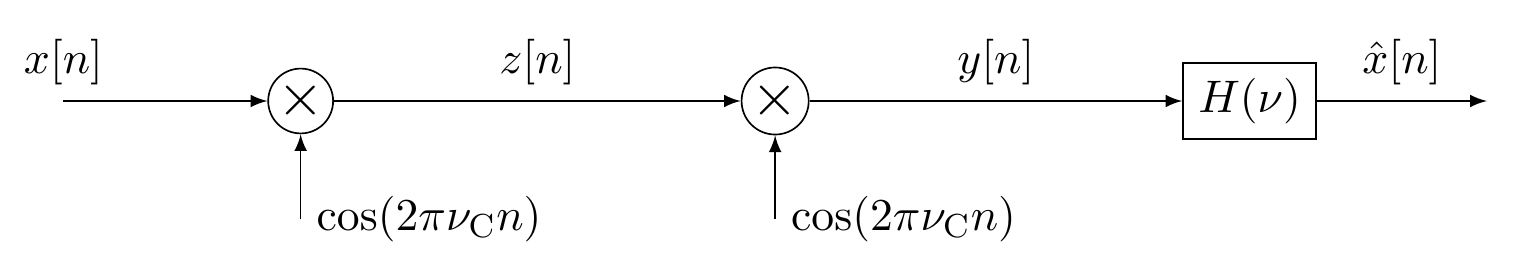
\includegraphics[width=0.83\columnwidth]{pic1.png}
  \end{center}
  \caption{Amplitude modulated discrete time system ~\cite{pek}.}
  \label{fig:pic1}
\end{figure}
\noindent
The problem is divided in two parts, one theory part which is intended to be solved first in order to be able to understand and solve the whole project.
In theory part the given signal is Fourier transformed and it's frequency domain is sketched and this parts can be found in the appendix of this report.
The second part of the problem is reconstruction of the original signal from the system. This is a demodulation implementation using Matlab.

\section{Theory}
Amplitude modulation is widely used in many communication system. In an AM a signal is multiplied  with a carrier wave with higher frequency than the signal it self. The amplitude of the carrier wave is varied in proportion to the signals amplitude as depicted in figure \ref{fig:am}
\begin{figure}[H]
  \begin{center}
    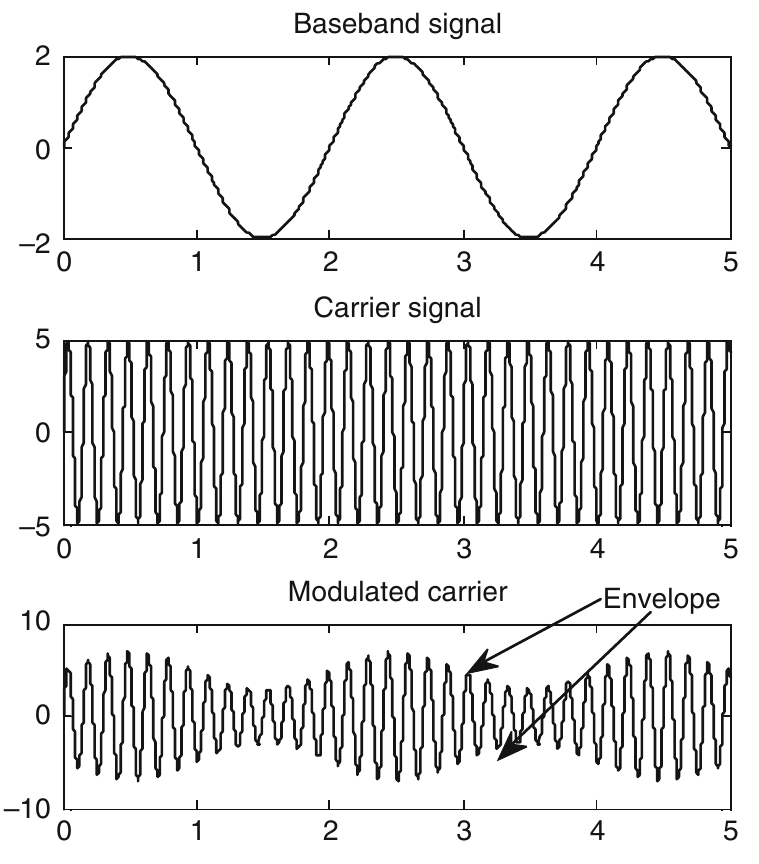
\includegraphics[width=0.83\columnwidth]{am2.png}
  \end{center}
  \caption{A signal modulated with carrier wave and it's modulation in analog domain~\cite{book2}}
  \label{fig:am}
\end{figure}
\noindent
With Amplitude modulation it's possible to share a communication medium among many concurrently signals~\cite{mit}.
However the big concern of data communication is data integrity. When the communication channel is established between sender and receiver the data can be disturbed by the unwanted noise. The good news is that by proper filtering the original data can be collected without any distortion.
The signal in equation (1) which is result of multiplication by the carrier wave as depicted in figure ~\ref{fig:pic1} has distortion of higher frequency than carrier frequency $\nu_c$.
\begin{equation}
y[n] = cos(2\pi \nu_cn)z[n]
\end{equation}
Using a low pass filter will remove the high frequency and the signal is filtered and hopefully the reconstruction of original signal $x[n]$ is possible and we are able to see the content.

\section{Procedures and Result}
\label{sec:praktik}

First the theory part of the problem is solved simply using some trigonometry math and Fourier transform. This part are dived in four sub task which is present in the appendix of the report.

\noindent
The second part of the problem is implementation and demodulation of the signal using Matlab.
The modulated signal which is given as signal vector $z[n]$ is called with the function $z = mkhwdata([860510xxxx])$ with the personal social security number as input parameter to the function. Before further implementation the frequency domain of the given signal is plotted in Matlab as in figure ~\ref{fig:spectrum1}.

\begin{figure}[H]
  \begin{center}
    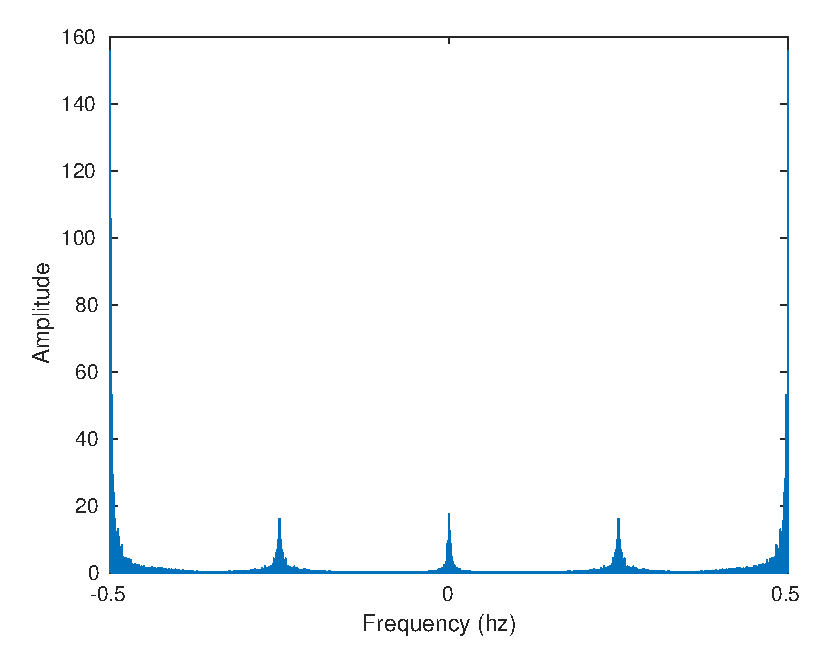
\includegraphics[width=0.9\columnwidth]{freq1corped.pdf}
  \end{center}
  \caption{Frequency spectrum of the signal before filtering.}
  \label{fig:spectrum1}
\end{figure}
\noindent
The given Matlab function $present\textunderscore image(z)$ is used to see the content of the signal as it's in figure \ref{fig:unfiltre_image}.
\begin{figure}[H]
  \begin{center}
    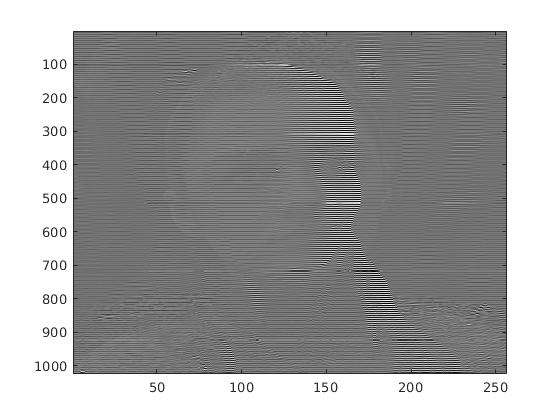
\includegraphics[width=0.83\columnwidth]{pic_sent.jpg}
  \end{center}
  \caption{The content of the signal before filtering.}
  \label{fig:unfiltre_image}
\end{figure}

\noindent
From frequency spectrum of the signal in figure ~\ref{fig:spectrum1} it's possible to read that the bandwidth is 0.5 Hz and the images are located at 0, 0.25hz and 0.5hz. A low pass filter of type $butter$ of order 9 and $filter$ is used to 
filter the noise of the signal. Both $butter$ and $filter$ are the built functions in Matlab. The input parameter of the filter $f_s$ is chosen to $f_s = 2 * 0.5 = 1 hz$ and the cut off frequency of the filter is chosen as $fc = \nu_c = 0.2 hz$. The image located at the center of the frequency spectrum in figure \ref{fig:spectrum1} was easy to recover by just applying the filter with chosen parameters. In order to filter the images located at 0.25hz and 0.5hz the signal is shifted by $cos(2*pi*0.25*n)$ and $cos(2*pi*0.5*n)$ to bring the images into the center and then applying the filter.
After the implementation of the filter the frequency spectrum and the content of the of the signal is plotted as shown below.

\begin{figure}[H]
  \begin{center}
    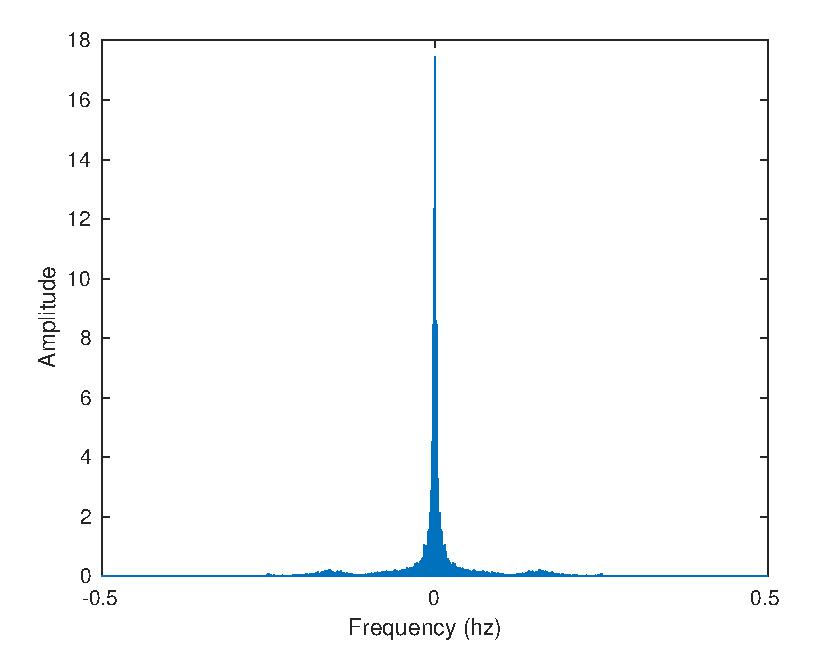
\includegraphics[width=0.9\columnwidth]{freq2corped.pdf}
  \end{center}
  \caption{The frequency spectrum of the signal after filtering.}
  \label{fig:spectrum2}
\end{figure}

\begin{figure}[H]
  \begin{center}
    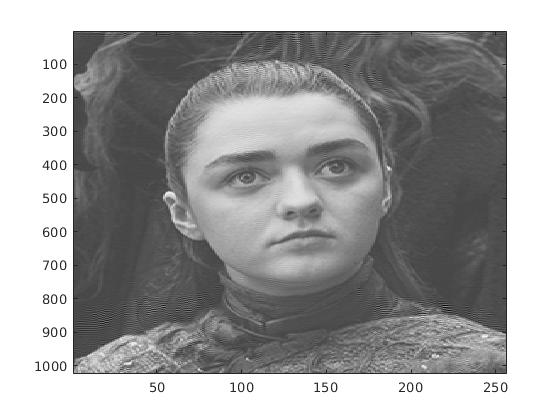
\includegraphics[width=0.9\columnwidth]{pic_recived.jpg}
  \end{center}
  \caption{The content of the signal at 0 Hz after filtering.}
  \label{fig:arya}
\end{figure}

\begin{figure}[H]
  \begin{center}
    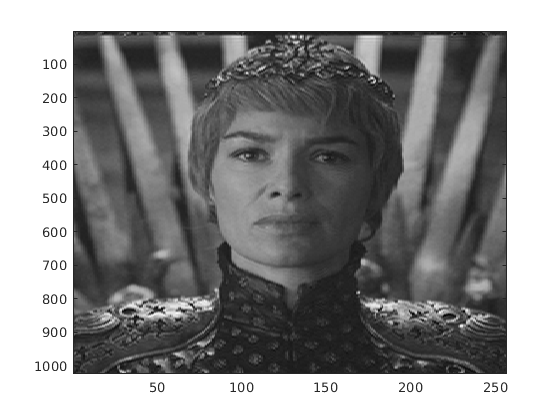
\includegraphics[width=0.9\columnwidth]{ceseiri.png}
  \end{center}
  \caption{The content of the signal at 0.25 Hz after filtering.}
  \label{fig:cersi}
\end{figure}

\begin{figure}[H]
  \begin{center}
    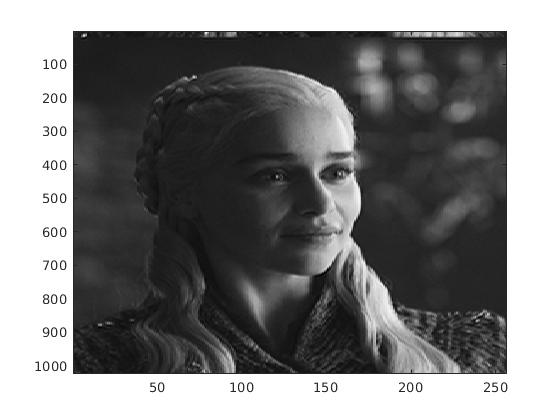
\includegraphics[width=0.9\columnwidth]{emilia.png}
  \end{center}
  \caption{The content of the signal at 0.5 Hz after filtering.}
  \label{fig:emilia}
\end{figure}


\section{Conclusions}
The demodulation of the signal is working as it's intended. It demodulate and filter the signal well but still there can be seen some shadow in the pictures. However it's possible to get more clearer signal perhaps with choosing the filter with shorter cut-off frequency. The built-in functions in Matlab is really amazing a lot of implementation time was saved by using those built-in functions instead of implementing those from the scratch.

\begin{thebibliography}{99}
\bibitem{pek}
KTH Elektro- och systemteknik, ”Hemuppgift 2, VT 2019
EQ1120 TIDSDISKRETA SIGNALER OCH SYSTEM "


\bibitem{mit}
\url{http://web.mit.edu/6.02/www/s2012/handouts.shtml}.
Modulation and demodulation Lecture 14 and chapter 14.

\bibitem{book}
GIRON-SIERRA, J. M. (2018). DIGITAL SIGNAL PROCESSING WITH MATLAB EXAMPLES, VOLUME 1: Signals and data, filtering, non-stationary signals, modulation.: SPRINGER.

\bibitem{book2}Das, A. (2010). Digital communication. New York: Springer, p.112.
\end{thebibliography}


\section*{Appendix}
\renewcommand{\thesubsection}{\Alph{subsection}}
\subsection{task 1}

\begin{equation}
\begin{aligned}
z[n] &= cos(2\pi \nu_cn)x[n] \\
&= \dfrac{1}{2} x[n]e^{j2\pi \nu_cn} + \dfrac{1}{2}x[n]e^{-j2\pi \nu_cn}
 \end{aligned}    
\end{equation}

The Fourier transform of (2) is 
\begin{equation}
\begin{aligned}
Z(\nu) = \dfrac{1}{2}X(\nu - \nu_c) + \dfrac{1}{2}X(\nu + \nu_c)
 \end{aligned}    
\end{equation}

\subsection{task 2}
The chosen frequency $\nu_c = 0.2$

\begin{figure}[H]
  \begin{center}
    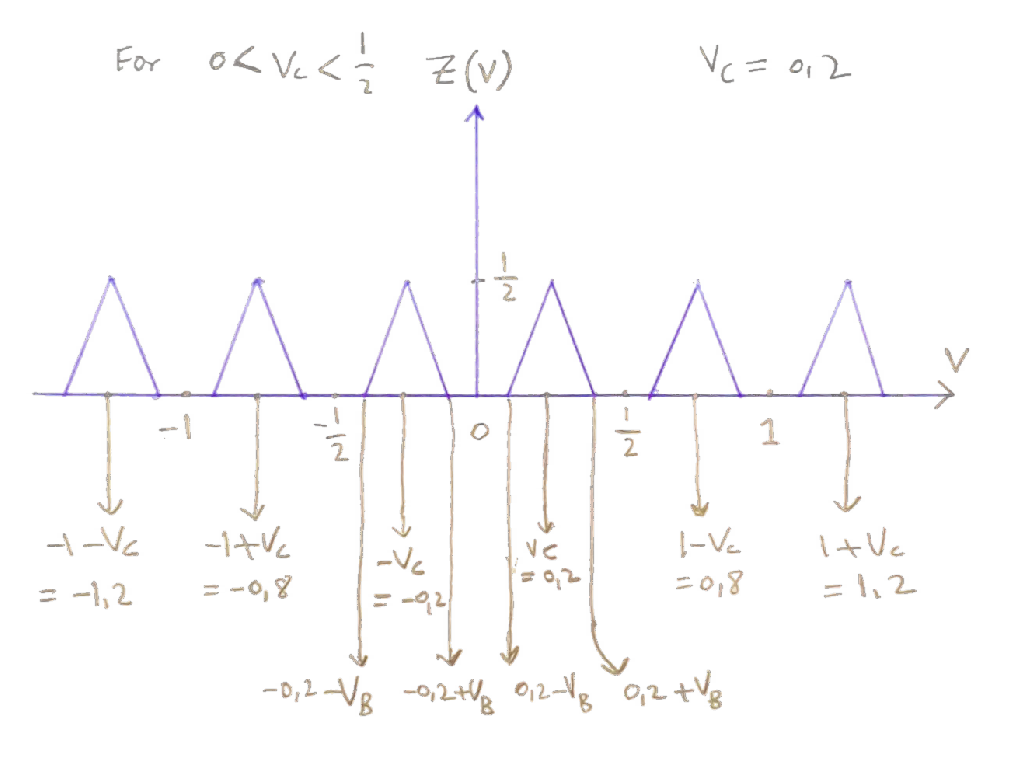
\includegraphics[width=0.83\columnwidth]{task2corped.pdf}
  \end{center}
  \caption{Discrete time Fourier transform of $Z(\nu)$.}
  \label{fig:prestanda}
\end{figure}

\subsection{task 3}
\begin{equation}
\begin{aligned}
z[n] &= cos(2\pi \nu_cn)x[n] \\
y[n] &= cos(2\pi \nu_cn)z[n] \\
&= cos^2(2\pi \nu_cn)x[n] \\
&= \big(\dfrac{1}{2} + \dfrac{1}{2}cos(4\pi \nu_cn)x[n]\big) \\
&= \dfrac{1}{2}x[n] +\dfrac{1}{4} x[n]e^{j4\pi \nu_cn} + \dfrac{1}{4}x[n]e^{-j4\pi \nu_cn}
 \end{aligned}    
\end{equation}
The Fourier transform of the equation (4) is 
\begin{equation}
\begin{aligned}
Y(\nu) = \dfrac{1}{2}X(\nu) + \dfrac{1}{4}X(\nu - 2\nu_c) + \dfrac{1}{4}X(\nu + 2\nu_c)
 \end{aligned}    
\end{equation}

\begin{figure}[H]
  \begin{center}
    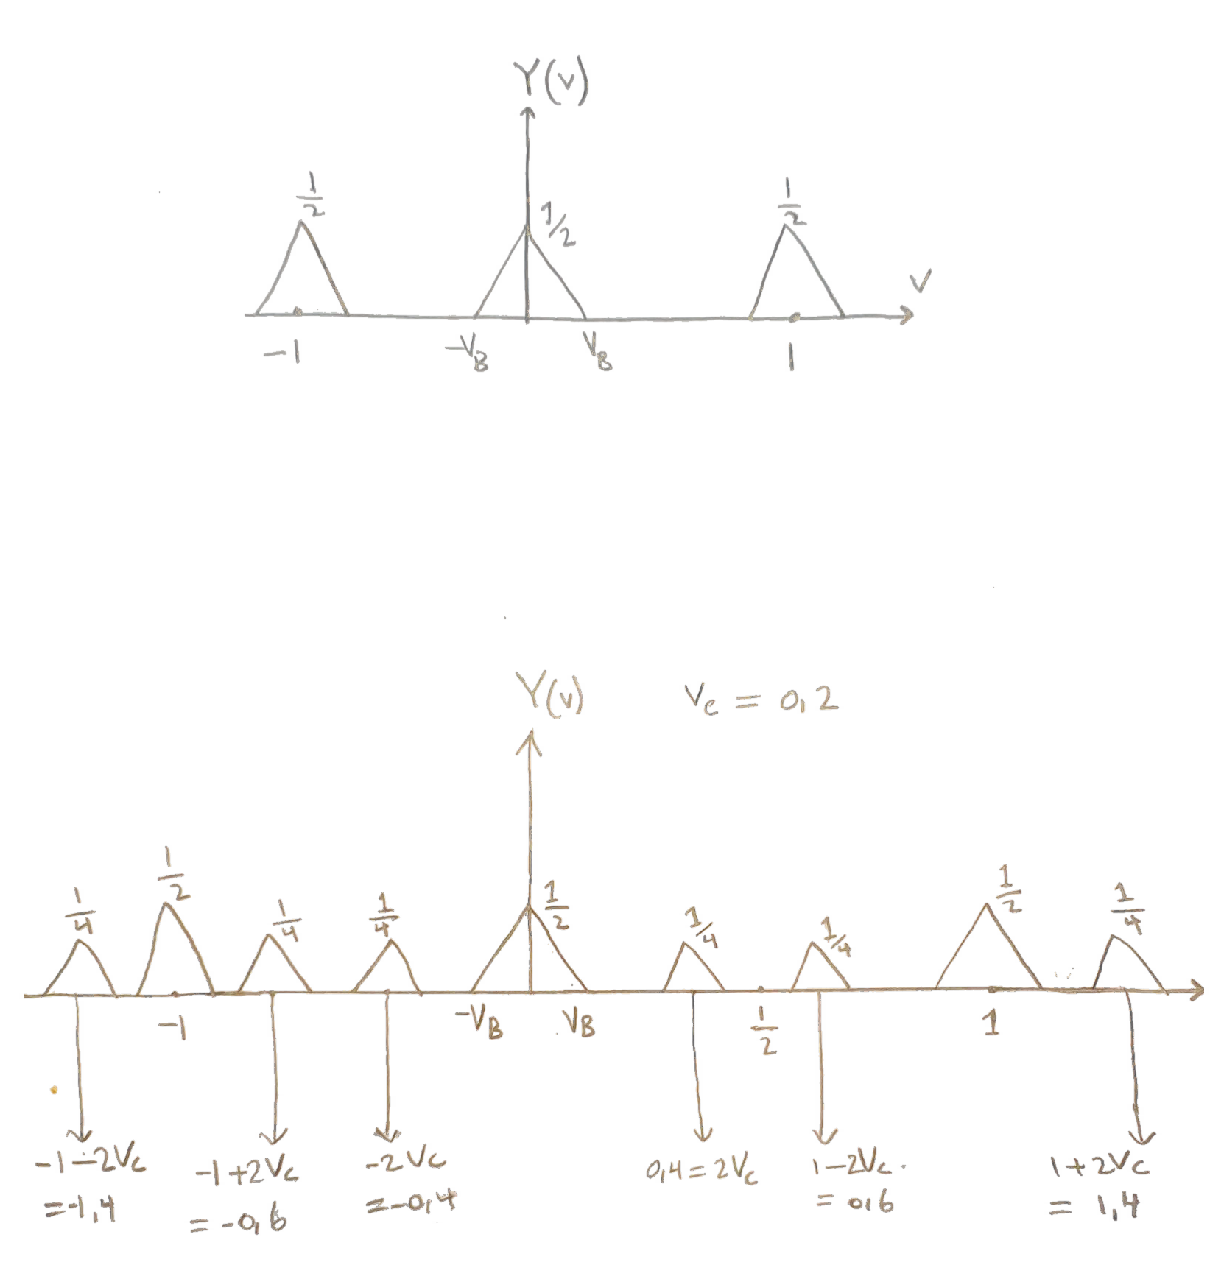
\includegraphics[width=0.83\columnwidth]{task3corped.pdf}
  \end{center}
  \caption{Discrete time Fourier transform of $Y(\nu)$.}
  \label{fig:prestanda}
\end{figure}
\subsection{task 4}
The carrier frequency $V_c >> V_B$
and we choose $H(\nu)$ as in figure~\ref{fig:prestanda} for example with a gain of 2 and select those frequencies than the $\hat{X}(\nu) = X(\nu)$. The inverse Fourier transform of this spectrum gives that $\hat{x}[n] = x[n]$ and the reconstruction of the original signal is possible.


\begin{figure}[H]
  \begin{center}
    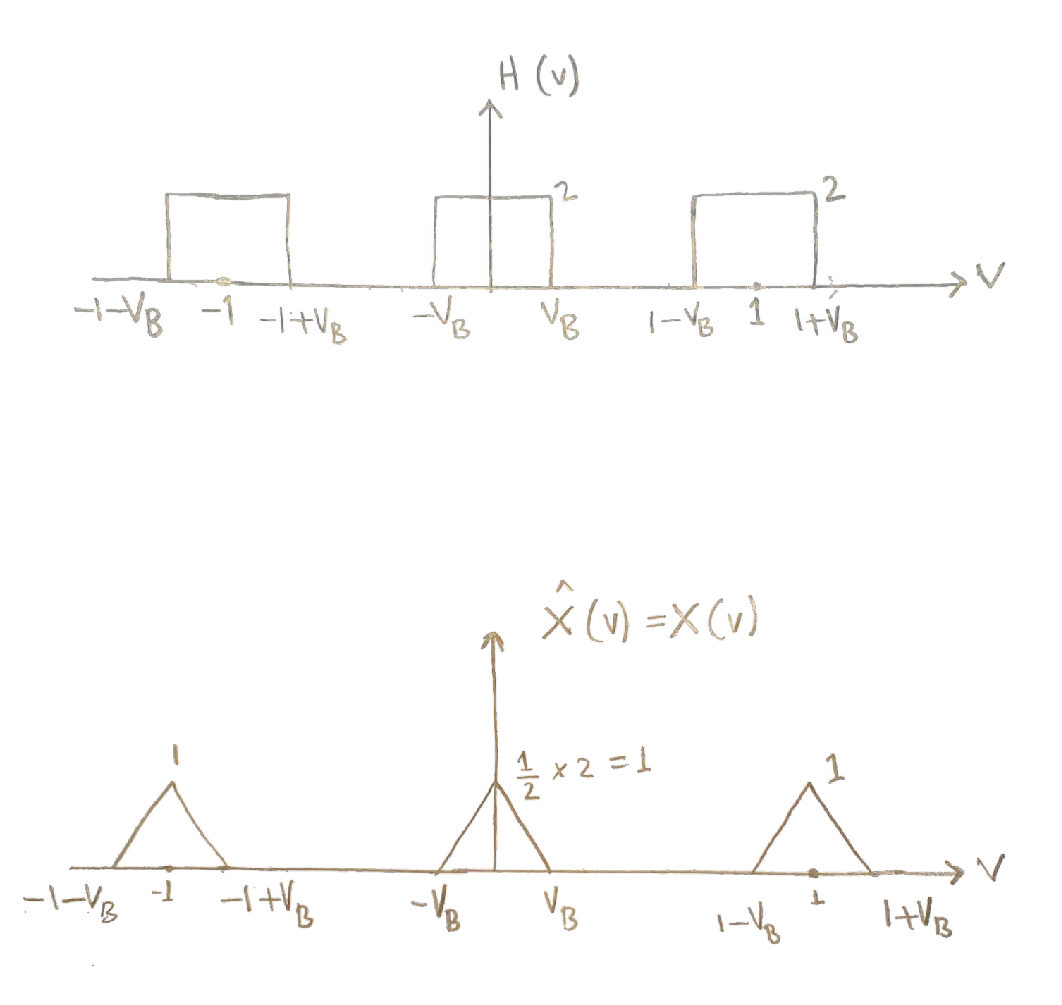
\includegraphics[width=0.83\columnwidth]{task1corped.pdf}
  \end{center}
  \caption{Discrete time Fourier transform of $X(\nu)$.}
  \label{fig:prestanda}
\end{figure}

\begin{figure}[H]
  \begin{center}
    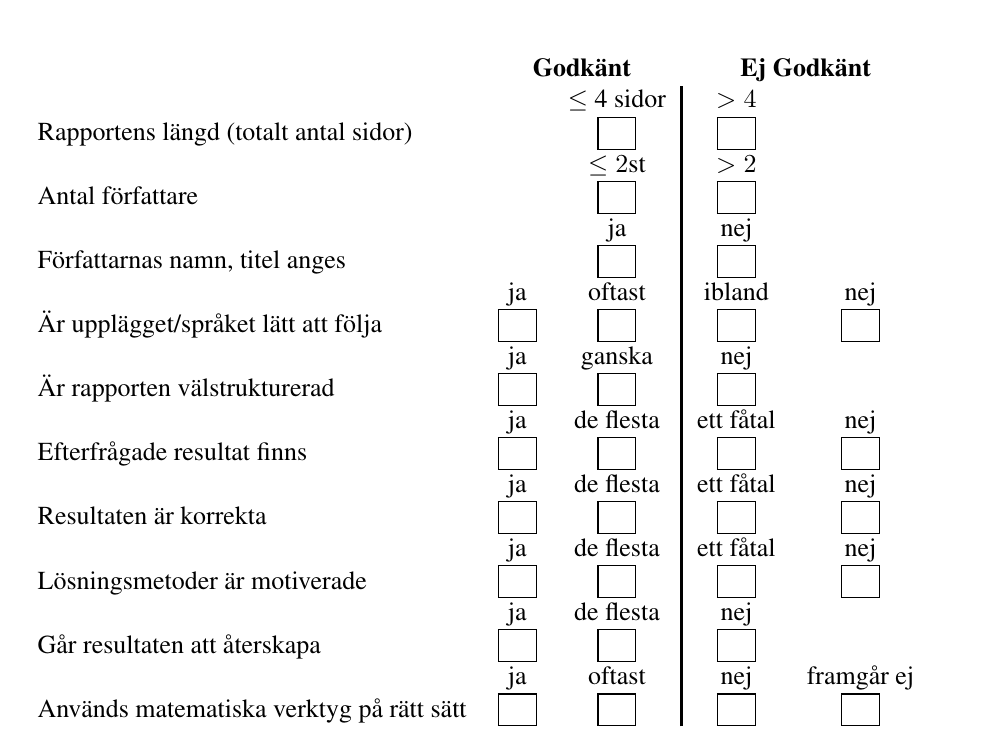
\includegraphics[width=\columnwidth]{evatab.png}
  \end{center}
  \caption{Evaluation template ~\cite{pek}.}
  \label{fig:evatable}
\end{figure}

\end{document}
